\documentclass[conference]{IEEEtran}

\usepackage {tikz}
\usetikzlibrary{positioning,fit,calc}
\tikzset{block/.style={draw, thick, align=center},   line/.style={-latex} }
\IEEEoverridecommandlockouts

\usepackage{cite}
\usepackage{amsmath,amssymb,amsfonts}
\usepackage{algorithmic}
\usepackage{graphicx}
\usepackage{textcomp}
\usepackage{xcolor}
\usepackage{float}
\usepackage{gensymb}
\usepackage{subcaption}
\usepackage{multicol}
\usepackage{ amssymb }
\graphicspath{{figs/}}
\def\BibTeX{{\rm B\kern-.05em{\sc i\kern-.025em b}\kern-.08em
    T\kern-.1667em\lower.7ex\hbox{E}\kern-.125emX}}
\usepackage{booktabs}
\begin{document}

\title{Hello world title\\
{\footnotesize }
\thanks{}
}

%\author{\IEEEauthorblockN{Carlo Jonas R. Cari\~no,test}
%\IEEEauthorblockA{\textit{Electrical and Electronics Engineering} \\
%\textit{University of the Philippines Diliman}\\
%Quezon City, Philippines \\
%}

\author{\IEEEauthorblockN{Carlo Jonas R. Cari\~no}
\IEEEauthorblockA{\textit{Electrical and Electronics Engineering Institute} \\
\textit{University of the Philippines Diliman}\\
Quezon City, Philippines \\
}
}

\maketitle

\begin{abstract}
put abstract hese
\end{abstract}

\begin{IEEEkeywords}
Robotics, Control, Systems
\end{IEEEkeywords}

\section{Introduction}
intro content
	
	\begin{figure}[H]
		\centering
		 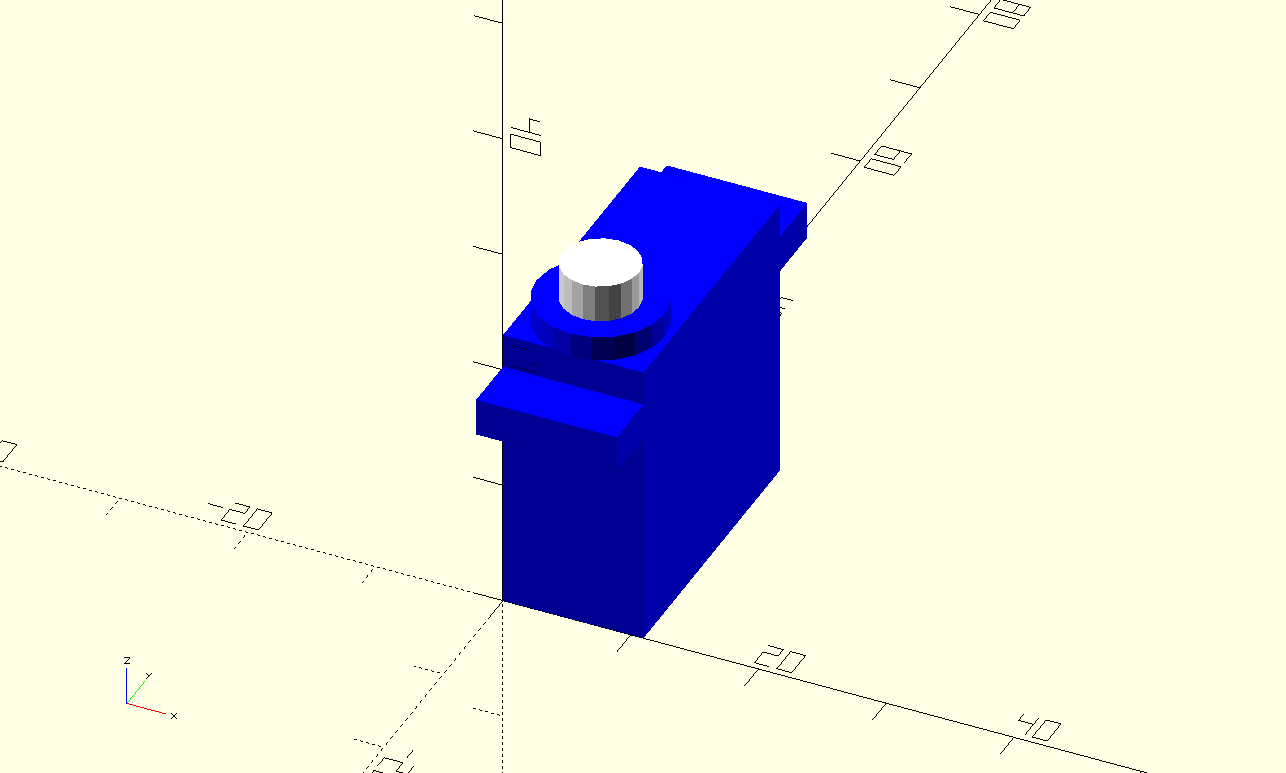
\includegraphics[width=0.75\linewidth]{./images/servo.png}
		 	\caption{A picture of a servo}
		  	%\label{fig:r}	
	\end{figure}	
	\subsection{Manufacturing}
		subsection
			\begin{equation}
			G_1 = m_1 g^T \frac{\partial A_0^1}{\partial \theta_1}\bar{p_1}
			\end{equation}
			
		
\section{Results and Discussion}
\label{results_section}
	\subsection{Positional Accuracy}
	\subsection{Geometric Accuracy}
	\subsection{Repeatability}
	
\section{Conclusion}
\label{conclusion_section}

\section{Recommendations}
\label{recommendations_section}

\newpage
%\bibliography{BibFile}

\newpage
\begin{appendices}
	\section{Preliminary Work}
	

\end{appendices}

\end{document}
